\documentclass[conference]{IEEEtran}

\usepackage[utf8]{inputenc}
\usepackage{amsmath}
\usepackage{graphicx}
\usepackage{tabularx}
\usepackage{adjustbox}
%\usepackage[colorinlistoftodos]{todonotes}
\usepackage{csquotes}
\usepackage{comment}
\usepackage{imakeidx}
%tabela
\usepackage{multirow}
\usepackage{xcolor}
\usepackage[margin=2.5cm]{geometry}
\usepackage{hyperref} %to show links
\usepackage{titling}
\usepackage[ddmmyyyy]{datetime}
\usepackage{setspace}
\usepackage{indentfirst}

%to define placement of tables and images in strict mode
%\usepackage{placeins}

\usepackage[style=ieee]{biblatex} 
\addbibresource{ref.bib}
\input{vars}
\linespread{1.2}

\begin{document}

\title{Implementing an HTML5 mobile simulation utilizing web workers}

\author{authored by\\
        Lari Alakukku (528362),
        Miika Rouvinen (356770),
        Ilkka Malassu (430463)}%

\makeatletter         
\def\@maketitle{
\begin{center}
{\Huge \bfseries \sffamily \@title }\\[4ex] 
Submitted on \@date\\
{\normalsize \@author}\\[4ex] 
%\@date\\[8ex]
\end{center}}
\makeatother


% make the title area
\maketitle

\begin{IEEEkeywords}
HTML5, web, workers
\end{IEEEkeywords}

%%%%%%%%%%%%%%%%%%%%%%%%%%%%%%%%%%%%%%%%%%%%%%%%%%%%%  
\begin{abstract}

Abstract of the paper here
 
\end{abstract}

\section{Introduction}
\label{chap:introduction}

In this section we present an introduction to the topic.

\section{Related Work}
\label{sec:soa}

Related research here.

\section{Implementation}

Here we present our implementation.

\subsection{Context} 
\label{sec:context}

Maybe a subsection if needed.

%%%%%%%%%%%%%%%%%%%%%%%%%%%%%%%%%%%%%%%%%%%%%%%%%%%%%  
\section{Evaluation}
\label{sec:sec2}

Here we present our evaluation of the implementation.
Example results in Figure \ref{fig:labeloffigure}. 

\begin{figure}[ht]
	\centering
	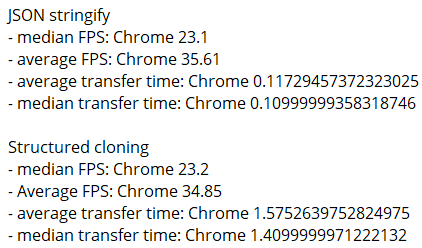
\includegraphics[scale=0.5]{figs/example.png}
	\caption{This is a figure}
	\label{fig:labeloffigure}
\end{figure}

\section{Conclusions}
\label{sec:conc}

We conclude our research paper here.

\printbibliography[title={References}]

\end{document}